% ============================================================================
%  AAAI-27 제출 논문 — 한국어 번역본 (내부 검토용)
%  영문 원본: main.tex  (두 파일은 구조가 1:1로 동일하게 유지됩니다)
%  컴파일: XeLaTeX 또는 LuaLaTeX (kotex 한글 지원)
% ============================================================================
\documentclass[letterpaper]{article} % DO NOT CHANGE THIS
\usepackage[submission]{aaai2027}  % DO NOT CHANGE THIS
\usepackage[hyphens]{url}  % DO NOT CHANGE THIS
\usepackage{graphicx} % DO NOT CHANGE THIS
\urlstyle{rm} % DO NOT CHANGE THIS
\def\UrlFont{\rm}  % DO NOT CHANGE THIS
\usepackage{natbib}  % DO NOT CHANGE THIS AND DO NOT ADD ANY OPTIONS TO IT
\usepackage{caption} % DO NOT CHANGE THIS AND DO NOT ADD ANY OPTIONS TO IT
\frenchspacing  % DO NOT CHANGE THIS
\usepackage{booktabs}
\usepackage{amsmath}
\usepackage{amssymb}
\usepackage{algorithm}
\usepackage{algorithmic}
\usepackage{kotex}   % 한글 지원 (XeLaTeX / LuaLaTeX 필요)

\pdfinfo{
/TemplateVersion (2027.1)
}

\setcounter{secnumdepth}{0}

\title{내결함성 강화학습을 위한\\
LLM 거버넌스 행동 제약}

\author{
    Anonymous Submission
}
\affiliations{
    Anonymous Submission
}

\begin{document}

\maketitle

% ============================ 초록 ============================
\begin{abstract}
심층강화학습(DRL)은 평균적으로는 휴리스틱과 대등하거나 능가할 수 있으나, 확률적
환경에서 학습된 정책은 종종 \emph{신뢰할 수 없다}: 고충실도 시뮬레이터의 내재적
비결정성으로 인해 동일하게 설정된 실행이 어떤 경우에는 우수한 정책으로 수렴하고 어떤
경우에는 치명적으로 실패한다. 기존 안전 RL 기법은 대부분 보상을 재정형하거나 정적
제약을 추가하는데, 우리는 이것이 불충분함을 보인다. 우리는 대형언어모델(LLM)을 정책
생성기가 아니라 기성 DRL 에이전트의 신뢰성을 높이는 \emph{적응형 거버넌스 모듈}로
취급할 것을 제안한다: 각 에피소드 후 로컬 호스팅 LLM이 실행의 KPI를 읽고 사람이 읽을
수 있는 안전 룰을 내보내며, 결정론적 계층이 이를 스텝별 행동 마스크로 컴파일한다.
우리는 이를 까다롭고 자원 임계적인 사례---실제 공장 데이터로 구축된 반도체 디지털
트윈에서의 긴급 로트 스케줄링---에 적용하며, 여기서 Pure DRL은 독립 실행의 60\%에서
실패한다($N{=}20$ 시드). 20개 시드에 걸쳐 제안 기법은 치명적 실패율을 60\%에서
15\%로, 평균 사이클 타임을 625\,s 감소시키며($p{<}0.01$), 그 이득은 여러 충돌 영역에
걸쳐 유지된다. 한 번에 하나의 설계 축을 제거하는 통제된 절제 연구는 \emph{왜}
작동하는지를 규명한다: 하드 마스크를 동등한 보상 정형화로 대체하면 거버넌스가 없는
DRL보다 \emph{더 나쁘며}($p{<}0.001$), 무조건적 마스킹은 45\,\%p 더 자주
실패하고($p{<}0.05$), 고정된 비적응 룰은 평균에 필적하지만 치명적 꼬리를 그대로
남긴다. 이득은 \emph{하드하고 맥락적이며 적응적인} 행동 제약에서 비롯되며, 이는 LLM이
제로샷으로, 로컬에서, 감사 가능하게 공급하는 속성이다. 우리는 이것이 LLM-over-DRL
거버넌스를 신뢰 가능한 RL을 위한 일반적 내결함성 메커니즘으로 재정의한다고 논한다.
\end{abstract}

% ============================ 1. 서론 ============================
\section{서론}

반도체 제조 라인은 확률적이고 비정상적(non-stationary)인 스케줄링 환경이다. 단일
디스패칭 결정은 재공품(WIP) 분포를 재편하고 수 시간 뒤의 사이클 타임에 영향을
미치므로, 시점 $t$의 행동은 귀속이 어렵고 고정 휴리스틱으로 최적화하기는 더 어려운
장기 영향을 수반한다 \citep{moyne2017,hu2019}. 이제 표준이 된 대응 방식은
\emph{디지털 트윈}---라인의 고충실도 이산사건 시뮬레이션---을 심층강화학습(DRL)과
결합하여 시뮬레이션 환경에서 직접 디스패칭 정책을 학습하는 것이다
\citep{waschneck2018,lee2025}. 그림~\ref{fig:drlbase}은 이 기본 결합을 나타낸다:
디지털 트윈은 현장 상태를 공급하고 디스패칭 행동을 받으며, 가치 기반 에이전트는
경험 재생을 통해 학습한다.

\begin{figure}[t]
  \centering
  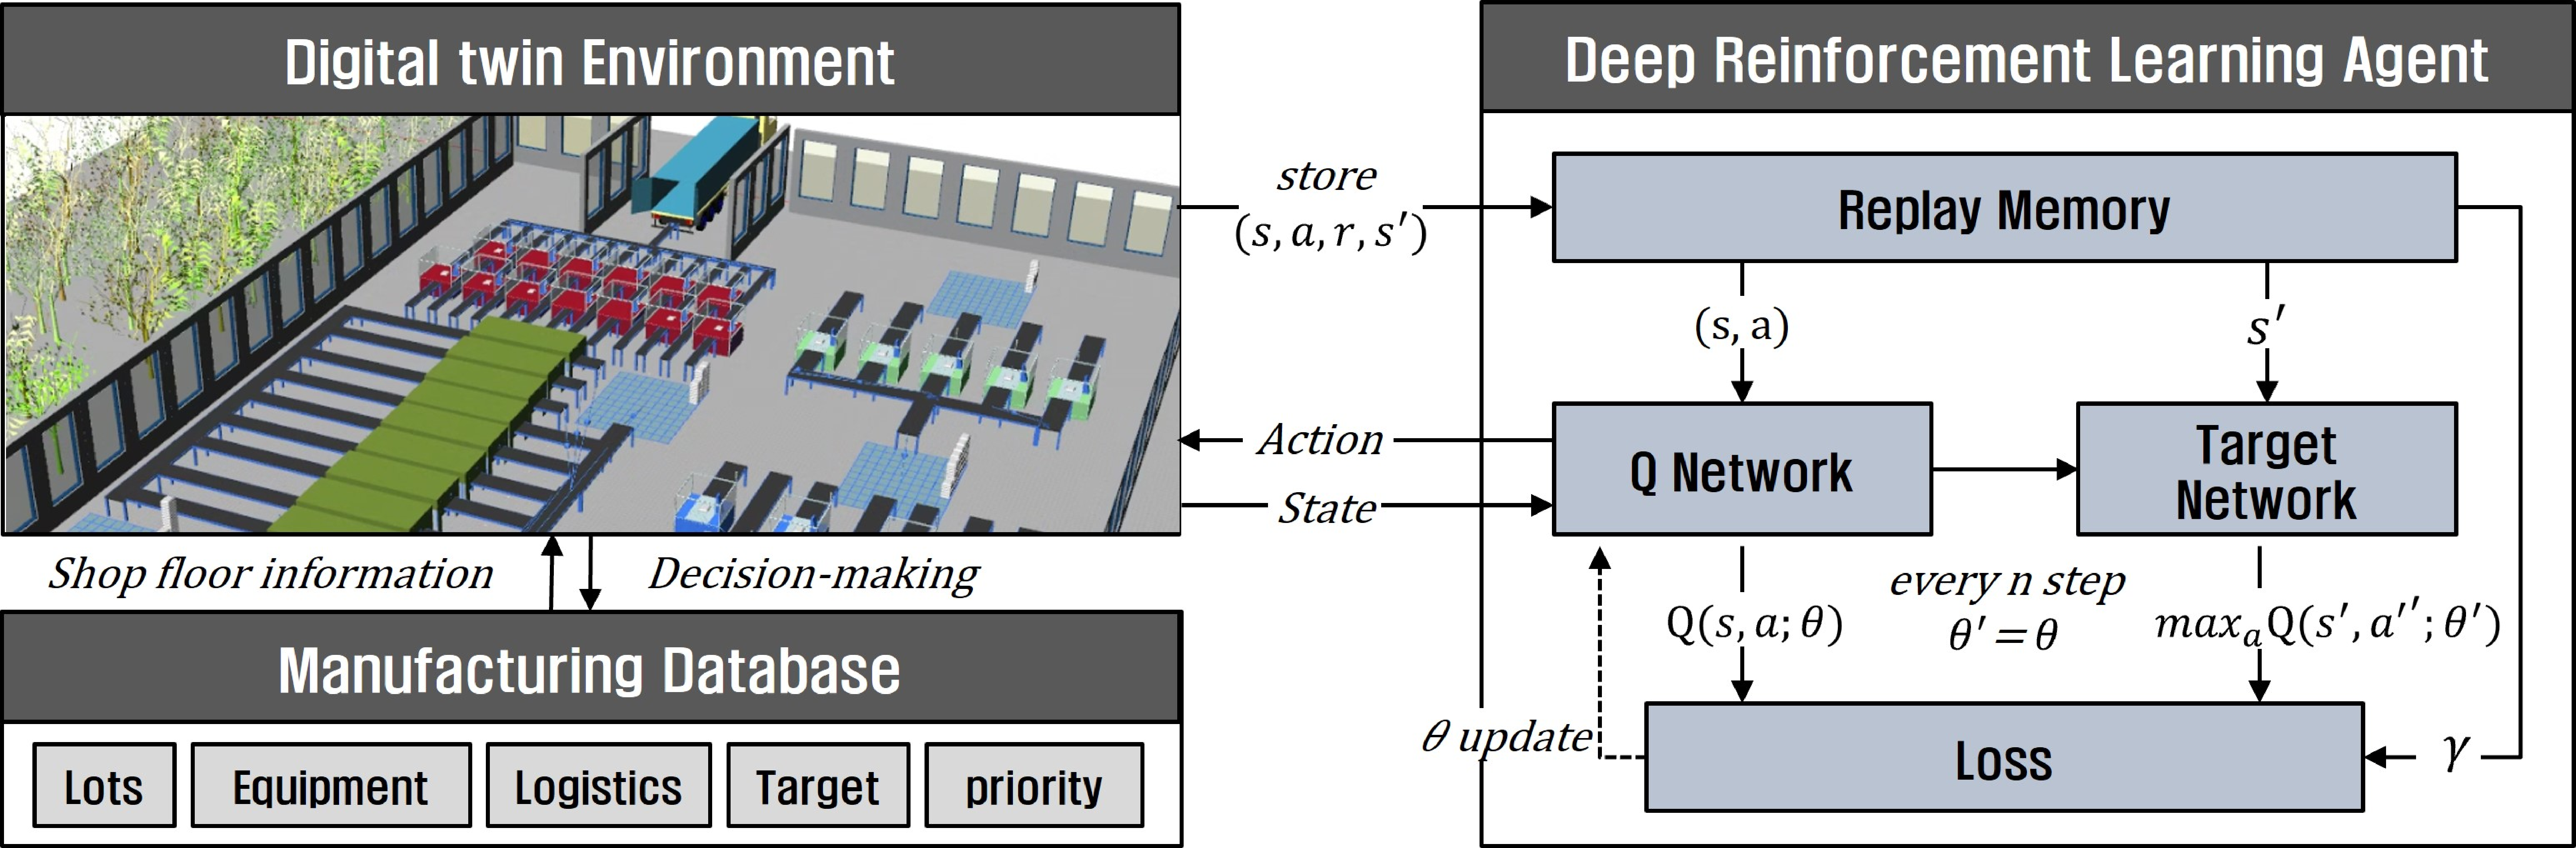
\includegraphics[width=0.92\columnwidth]{Figures/fig_drlbaseline.pdf}
  \caption{기본 DRL 스케줄링 루프. 디지털 트윈이 학습 환경 역할을 하며, 에이전트는
  현장 상태 $s$를 관측하고 디스패칭 행동 $a$를 선택하여 보상 $r$을 받고 Q-네트워크를
  갱신한다. 이 결합은 평균적으로는 효과적이지만, 본 논문이 보이듯 실행마다 신뢰할 수
  없다.}
  \label{fig:drlbase}
\end{figure}

고무적인 평균 성능에도 불구하고, 비용·수율이 중요한 제조에 DRL을 적용하면 문헌이
거의 정량화하지 않은 문제가 드러난다: 학습된 정책이 \emph{실행마다 신뢰할 수
없다}는 점이다. 디지털 트윈이 내부적으로 비결정적이기 때문에, 동일하게 설정된 학습
실행이 한 번은 고품질 정책으로 수렴하고 다른 한 번은 치명적으로 실패한다. 이러한
취약성은 긴급 로트 충돌이 빈번할 때 가장 두드러진다: 소수의 고우선순위 로트가
라인을 빠르게 통과해야 하지만, 이들이 병목에서 실질적 경합을 일으킬 만큼 많아지면
긴급 처리에 대한 보상 신호가 잡음이 많아지고 수렴이 운에 좌우된다. 따라서 핵심
질문은 신뢰성 관점에서 보면, 스케줄러는 \emph{간헐적 결함}(intermittent fault)을
보인다: 명목상 동일한 조건에서 가끔 실패 스케줄을 낸다. 따라서 핵심 질문은 ``어떻게
DRL을 평균적으로 더 빠르게 만들 것인가?''가 아니라 \emph{내결함성}의 질문이다---관측·제어
불가능한 비결정성의 원천이 치명적 정책으로 발현되지 않게 어떻게 막을 것인가? 표준 안전
RL 수단인 보상 정형화와 정적 안전 제약은 이 간헐적 실패 양상을 직접 겨냥하지 못하며,
우리는 그것들이 여기서 불충분함을 보인다.

이 비신뢰성의 대가는 자원 임계적 공장에서 크다. 많은 로트는 \emph{품질시간}(Q-time)
제약---연속 공정 단계 사이의 최대 허용 간격으로, 이를 넘기면 수율 보전을 위해
스크랩되거나 재작업되어야 함---의 지배를 받으며 \citep{kim2018qtime}, 이러한 시간 임계
로트가 바로 스케줄러가 우선 처리해야 할 대상이다. 신뢰할 수 없는 정책이 이들의 사이클
타임을 폭주시키면 Q-time 창이 위반되어 그 로트에 체화된 에너지·초순수·소재가
낭비된다 \citep{boyd2012,gutowski2009}. 따라서 치명적 스케줄은 느린 평균이 아니라
간헐적이고 비가역적인 손실이며---바로 그렇기에 평균을 깎는 것이 아니라 실패
\emph{꼬리}를 제거하는 것이 중요하다.

한 가지 해법은 에이전트를 올바른 긴급 로트 처리로 유도하는 외부 거버너를 두는
것이다. 대형언어모델(LLM)은 매력적인 후보다: 도메인 지식을 자연어로 인코딩하며,
태스크별 학습 없이 사람이 읽을 수 있는 룰을 생성할 수 있다. 선행 연구는 LLM을 목표
분해 \citep{du2023}, 상호작용 환경에서의 정책 그라운딩 \citep{carta2023}, 지시문의
코드 변환 \citep{liang2023}에 활용했다. 그러나 단순히 ``LLM + DRL''이 지표를
개선한다는 것을 보이는 것만으로는 핵심 과학적 질문에 답하지 못한다: \emph{설계의
무엇이 실제로 이득을 만드는가?} LLM의 적응적 추론인가, 행동 공간을 제약하는 행위
자체인가, 갱신 빈도인가, 아니면 단지 어떤 외부 신호의 주입인가? 이 요인들을
분해하지 않으면, 그러한 시스템은 신뢰·재현·전이가 어렵다.

본 논문은 통제된 연구를 통해 이 질문에 답한다. 우리는 3계층 계층적 강화학습(HRL)
프레임워크---에피소드 룰을 생성하는 LLM 전략가(L2), 이를 행동 마스크로 컴파일하는
결정론적 안전 계층(L1), Rainbow DQN 전술 에이전트(L0)---를 채택한 뒤, 보상 함수를
고정한 채 각 설계 차원을 체계적으로 절제한다. 실험은 $N{=}20$개 독립 시드를
사용하며, 이는 이 분야에서 일반적인 수준보다 상당히 큰 신뢰성 표본으로, 단일 실행
평균이 아니라 실패율 분포를 보고한다 \citep{henderson2018,agarwal2021}. 우리는 반도체
스케줄링을 까다롭고 자원 임계적인 테스트베드로 다루지만, 우리가 겨냥하는
현상---환경 비결정성 하의 치명적 정책 실패---과 제안하는 거버넌스 해법은 이에
특화되지 않는다(논의 절).

우리의 발견은 세 가지 설계 축을 따라 두드러진다. 첫째, 제안 기법은 Pure DRL 대비
치명적 실패율을 60\%에서 15\%로, 평균 사이클 타임을 625\,s 감소시킨다($p{<}0.01$).
둘째, \emph{하드} 행동 마스크를 동등한 \emph{보상 정형화} 항으로 대체하면 성능이
\emph{거버넌스 없는 DRL보다 더 나빠진다}($p{<}0.001$): 이득은 보상을 미세 조정하는
데 있는 것이 아니라 안전하지 않은 행동을 가지치기하는 데 있다. 셋째, 맥락을
고려하지 않은 \emph{무조건적} 무작위 마스크는 제안 기법보다 45\,\%p 더 자주
실패하여($p{<}0.05$), 제약이 존재한다는 사실이 아니라 제약이 \emph{언제} 발동하는가가
중요함을 보인다. 넷째, 고정된 비적응 룰과의 비교는 그것이 우리의 \emph{평균} 사이클
타임에 필적하면서도 여전히 실행의 60\%에서 실패함을 보여, 꼬리를 제거하려면 적응적
수정이 필요함을 확인한다. 이들은 핵심 요소를 함께 분리한다: \emph{하드하고
맥락적이며 적응적인} 행동 제약.

\noindent 본 논문의 기여는 다음과 같다.
\begin{itemize}
\setlength\itemsep{0.15em}
\item \textbf{내결함성 RL을 위한 LLM 거버넌스.} LLM을 정책 생성기가 아니라 적응형
거버넌스 모듈로 사용하여, 시뮬레이터 비결정성이라는 간헐적 결함을 하드하고 KPI 조건부인
행동 제약으로 기성 DRL 에이전트를 견고화함으로써 견딘다.
\item \textbf{블랙박스가 아닌 메커니즘.} 통제된 단일 축 절제 연구가 세 직교
속성---\emph{하드}, \emph{맥락적}, \emph{적응적}---을 이득의 공동 책임 요소로
식별하여, 보상 정형화·무조건적 마스킹·고정 룰과 무엇이 다른지를 분리한다.
\item \textbf{평가 기준으로서의 실패율.} 대규모($N{=}20$ 시드)로 DRL의 치명적 실패
분포를 규명하고, 평균 성능이 아니라 실패율 감소를 안전 임계 RL의 지표로 채택한다---처리량
손실 없이 실패율을 60\%에서 15\%로($p{<}0.01$), 충돌 영역에 걸쳐 일관되게 낮춘다.
\item \textbf{자원 임계적 사례 검증.} 실제 공장 데이터로 구축된 반도체 디지털
트윈에서의 긴급 로트 스케줄링으로 접근법을 검증하고, 동일한 레시피가 드물고 비용이 큰
사건으로 인해 평균보다 신뢰성이 더 중요한 다른 도메인으로 전이되는 이유를 논의한다.
\end{itemize}

% ============================ 2. 관련 연구 ============================
\section{관련 연구}
\label{sec:related}

\paragraph{스케줄링을 위한 DRL과 디지털 트윈.}
RL은 장기·재진입(re-entrant) 특성으로 인해 정적 룰 기반 정책이 어려움을 겪는
반도체 디스패칭의 대안으로 적용되어 왔다 \citep{waschneck2018,hu2019}. 일반적인
방식은 이산사건 디지털 트윈을 가치 기반 에이전트와 결합하여 디스패칭 룰을
선택하게 하는 것이다 \citep{lee2025}. 우리는 전술 계층에 Rainbow DQN을 채택한다
\citep{hessel2018}. 이 문헌은 압도적으로 소수 실행에 대한 \emph{평균} 성능을
보고하며, 단일 불량 스케줄이 수율에 치명적 손실을 초래할 때 정작 중요한 속성인
\emph{신뢰성}---독립 학습 간 결과 분포, 즉 \emph{신뢰 가능한} RL의 관심사---을 거의
분석하지 않는다. 우리는 $N{=}20$ 시드로 이 분포적 관점을 전면화한다.

\paragraph{희소 보상과 외부 유도.}
보상받아야 할 사건이 드물면 에이전트는 신호를 거의 받지 못하고 이를 무시하는 지역
최적점에 빠질 수 있다 \citep{pathak2017}. 고전적 대응은 보상 정형화
\citep{ng1999}와 내재적 동기 \citep{pathak2017}다. 전자는 보상을 증강하지만
비정상적이고 왜곡된 학습 목표를 만들고, 후자는 \emph{어떤} 드문 행동을 학습할지
보장하지 못한다. 우리는 대신 외부 거버너를 통해 행동 공간을 제약하여 보상은 그대로
둔다---행동 마스킹을 통한 안전 RL의 한 형태다 \citep{garcia2015}. 우리의 절제
연구는 이러한 대안들을 직접 대조하여 행동 제약 경로가 결정적임을 보인다.

\paragraph{강화학습을 유도하는 LLM.}
LLM은 RL에 고수준 지식을 주입하는 데 사용되어 왔다: 장기 목표 분해
\citep{du2023}, 온라인 RL을 통한 정책 그라운딩 \citep{carta2023}, 지시문의 실행
가능 코드 변환 \citep{liang2023}. 보완적 흐름은 안전을 형식적 제약으로
인코딩한다(예: 지시문을 시간 논리로 변환하여 안전하지 않은 행동을 가지치기)
\citep{hasanbeig2020}. 우리 프레임워크는 두 가지 점에서 다르다. 첫째, 거버넌스가
\emph{연속적이고 KPI 기반}이다: LLM이 매 에피소드 라인 상태를 재평가하고 룰을
수정하며, 정적 초기 안내를 제공하지 않는다. 둘째, \emph{빈도 분리}되어 있다: LLM은
에피소드 시간 척도에서 동작하고, 경량 안전 에이전트가 밀리초 디스패치 척도에서
룰을 집행한다. 이는 고수준 관리자가 저수준 작업자의 목표를 설정하는 계층적 RL과
부합한다 \citep{vezhnevets2017}. 결정적으로, LLM 안내가 도움이 된다고만 보고하는
선행 연구와 달리, 우리는 하드함·맥락·적응성의 기여를 \emph{절제}하여 무엇이 이득을
책임지는지 규명한다.

% ============================ 3. 방법 ============================
\section{3계층 거버넌스 아키텍처}
\label{sec:arch}

\begin{figure}[t]
    \centering
    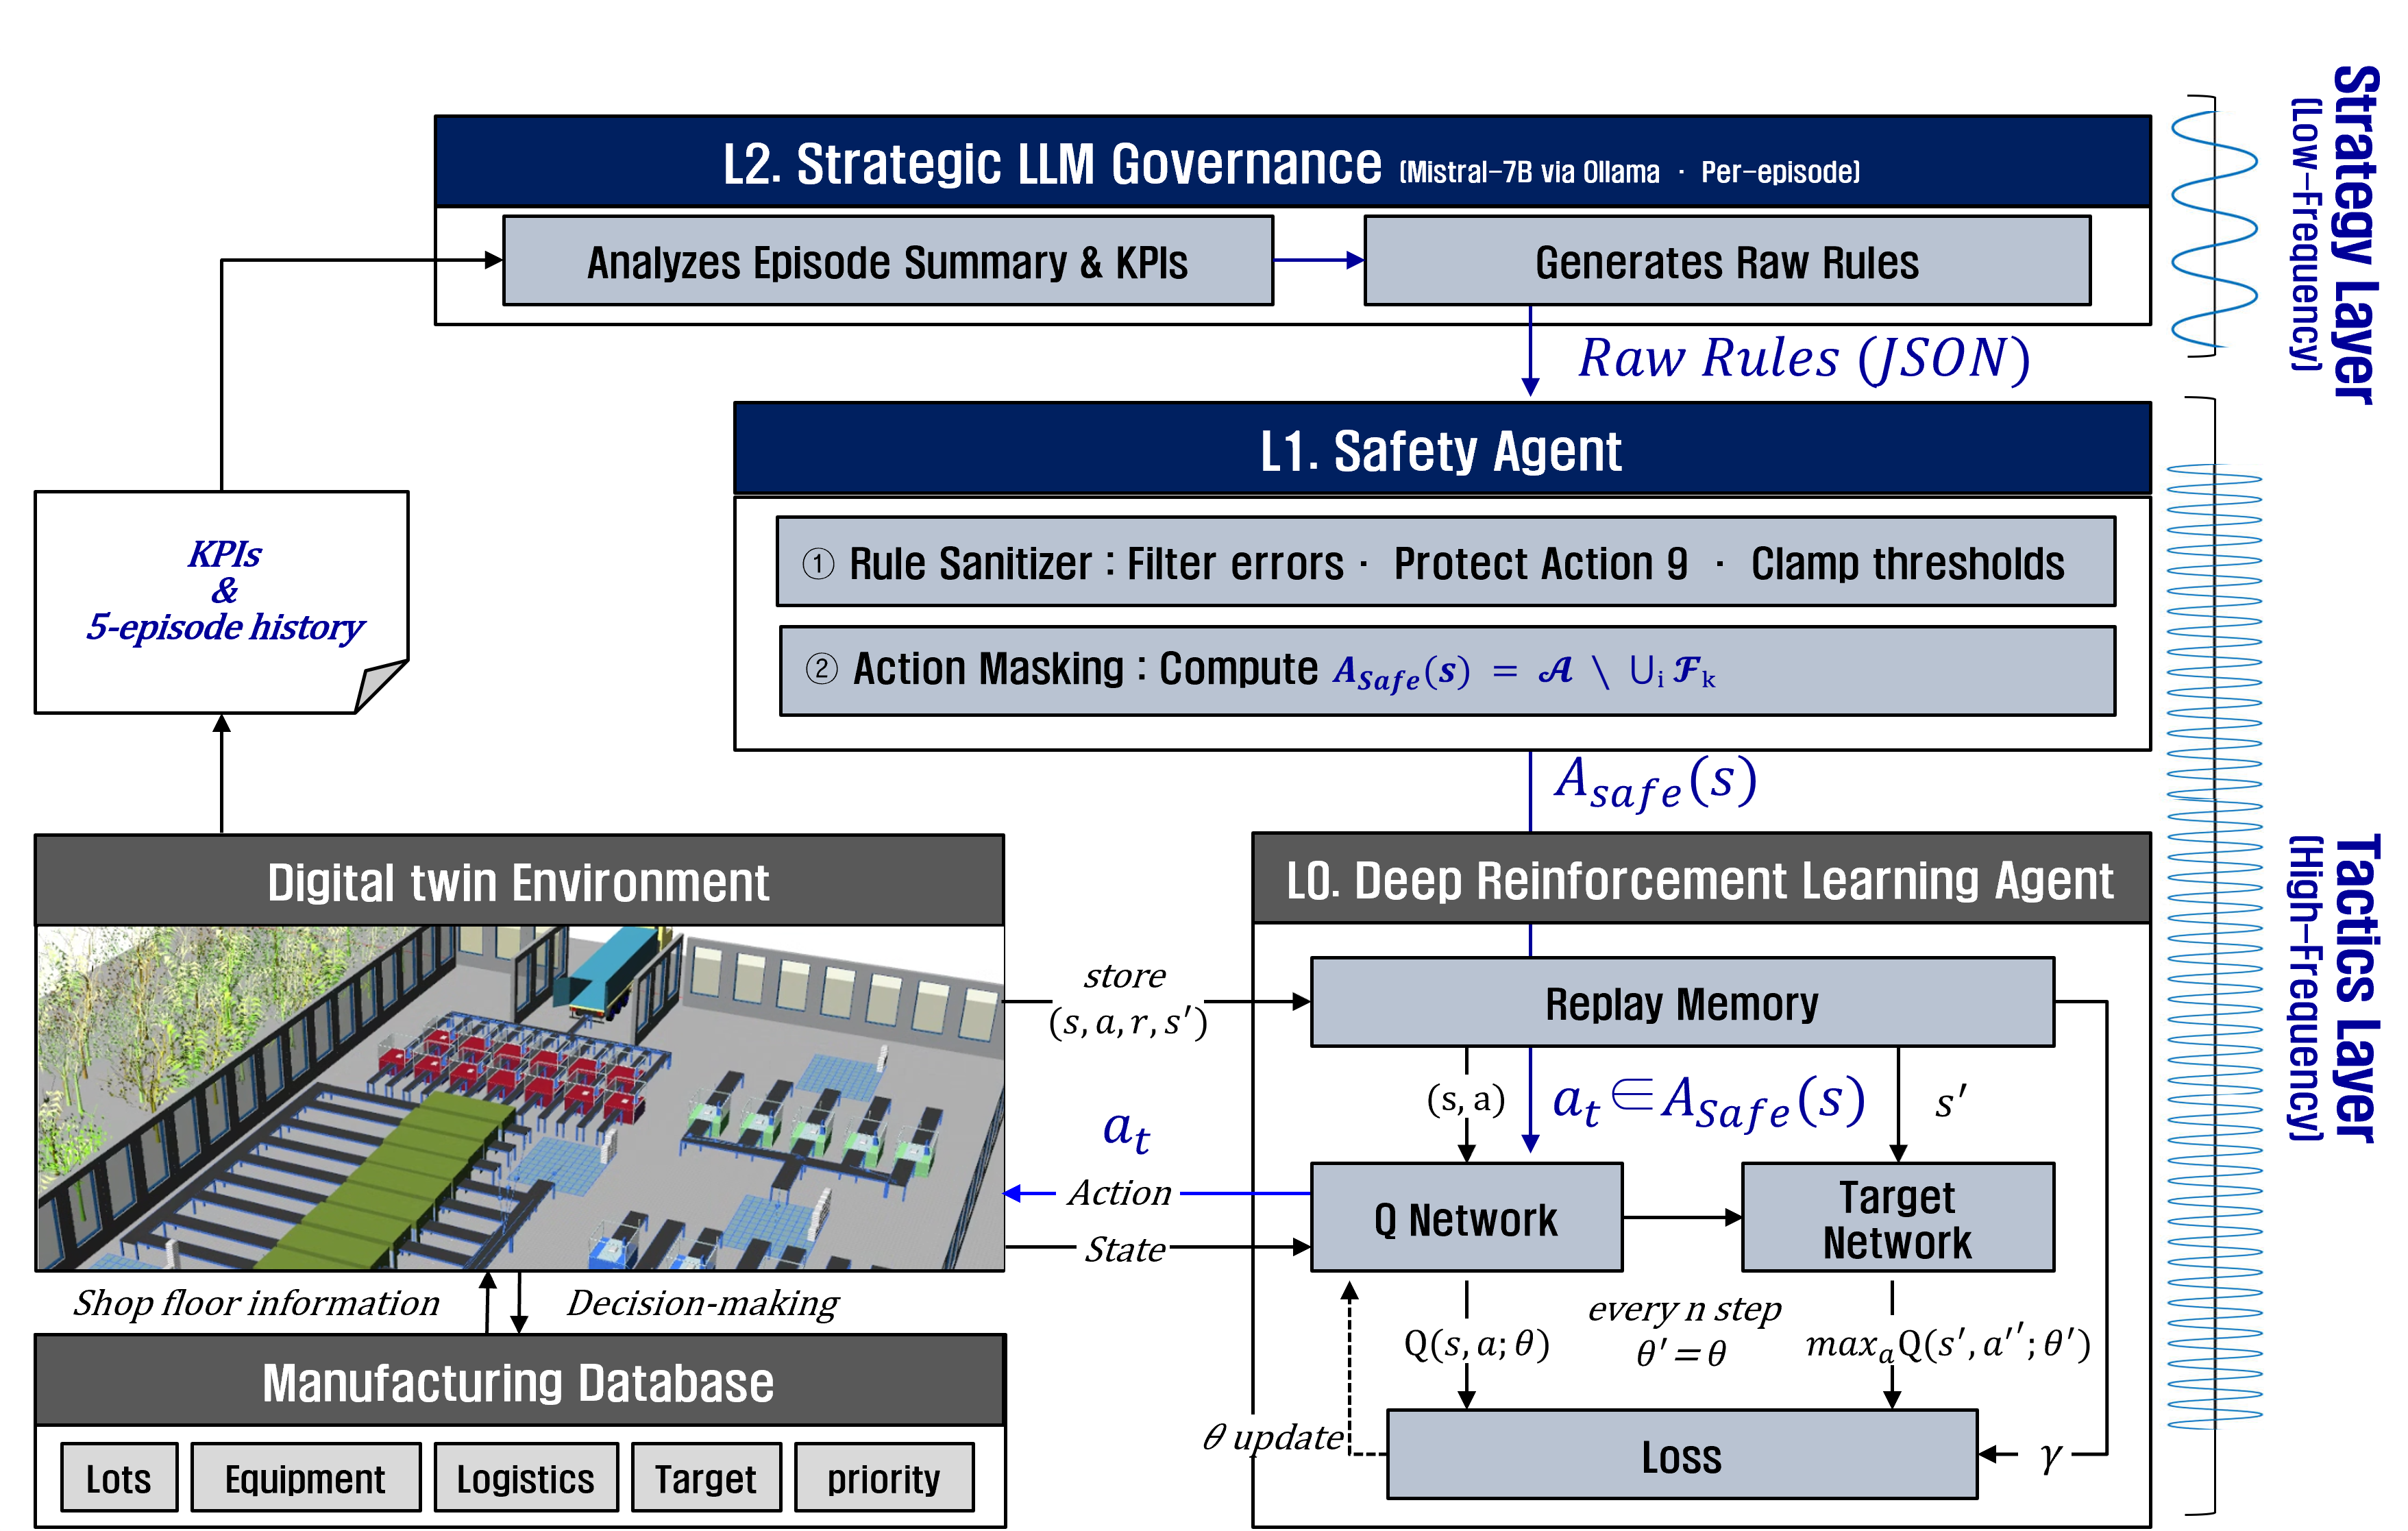
\includegraphics[width=0.96\columnwidth]{Figures/fig_architecture.png}
    \caption{3계층 거버넌스 아키텍처. L2(로컬 호스팅 LLM)는 KPI로부터 에피소드 안전
    룰을 생성하고, L1(안전 에이전트)은 내장 새니타이저로 이를 검증한 뒤 스텝별 행동
    마스크를 집행하며(식~\ref{eq:mask}), L0(Rainbow DQN)는 허용된 행동 중 가치가
    가장 높은 행동을 선택한다(식~\ref{eq:constrained}). 하드 제약 하한선은 거버넌스가
    생산 목표 달성을 희생하지 못하도록 한다.}
    \label{fig:arch}
\end{figure}

그림~\ref{fig:arch}은 프레임워크를 요약하며, 세 계층에 걸쳐 \emph{전략}과
\emph{전술}을 분리한다. 세 가지 원칙이 이를 선행 LLM 유도 RL과 구별한다.
\textbf{(i) 빈도 분리}: LLM은 에피소드당 한 번 추론하고 결정론적 에이전트가 매 밀리초
척도 스텝에서 룰을 집행하여, LLM의 지식과 실시간 제어의 지연 예산 사이 긴장을
해소한다. \textbf{(ii) 보상이 아닌 행동 제약에 의한 거버넌스}: LLM은 안전하지 않은
행동을 \emph{가지치기}하고(식~\ref{eq:mask}) 보상은 손대지 않아, 보상 정형화가
도입하는 비정상적 목표를 피한다---절제 연구가 이 구분이 결정적임을 보인다.
\textbf{(iii) 구성에 의한 안전}: 결정론적 새니타이저와 하드 생산 하한선이 불완전한
모델과 제어 루프 사이에 위치하여 잘못된 룰이 안전을 위반하거나 처리량을 희생할 수
없게 하며, 각 룰은 감사 가능한 자연어 근거를 수반한다. 아래에서 각 계층을 상술한다.

\paragraph{L2 -- 전략적 거버넌스(로컬 LLM).}
각 학습 에피소드 후, 로컬 호스팅 LLM은 에피소드의 집계 KPI(긴급 로트 수와 생산
부족률)와 5 에피소드 롤링 히스토리를 받아, (i) 성능 추세 분석, (ii) 지배적 병목
진단, (iii) 0개 이상의 안전 룰 생성---각 룰은 (지표, 연산자, 임계값, 금지 행동)의
튜플---을 수행하도록 프롬프트된다. LLM은 구조화된 JSON 응답을 반환하며 각 룰에 근거를
명시하고, 위의 빈도 분리 설계에 따라 에피소드당 한 번 호출된다.

\paragraph{L1 -- 안전 집행.}
경량 안전 에이전트는 룰 집합 $\mathcal{R}=\{r_1,\dots,r_K\}$를 받아 매 스텝
집행한다. 내장 새니타이저가 먼저 각 룰을 검증하여, 논리가 반전된 술어를 버리고,
긴급 로트 행동이 억제되지 않도록 보호하며, 임계값을 스텝별 척도로 클램핑한다.
검증된 각 룰 $r_k=(m_k,\odot_k,\theta_k,\mathcal{F}_k)$는 지표 $m_k$, 연산자
$\odot_k\in\{>,\geq,<,\leq\}$, 임계값 $\theta_k$, 금지 행동 집합
$\mathcal{F}_k\subseteq\mathcal{A}$를 지정한다. 상태 $s$에서의 \emph{안전 행동
집합}은
\begin{equation}
  A_{\text{safe}}(s)=\mathcal{A}\setminus
  \bigcup_{k:\,m_k(s)\,\odot_k\,\theta_k}\mathcal{F}_k,
  \label{eq:mask}
\end{equation}
이며 L0는 다음을 선택한다.
\begin{equation}
  a^{*}=\arg\max_{a\in A_{\text{safe}}(s)} Q(s,a;\theta).
  \label{eq:constrained}
\end{equation}
$A_{\text{safe}}(s)=\emptyset$이면 폴백이 제약 없는 탐욕적 행동으로 되돌려 교착을
방지한다. 안전 에이전트는 결정론적이고 감사 가능하다.

\paragraph{L0 -- 전술 에이전트(Rainbow DQN).}
Rainbow DQN 에이전트 \citep{hessel2018}는 $A_{\text{safe}}$ 내에서 동작한다.
21차원 상태(정규화 시간, 패밀리별 버퍼 점유율, 디바이스별 생산 부족, 리드타임 위험
통계, 임계 공정의 긴급 로트 수)를 관측하고 10개 디스패칭 행동 중 하나를 선택한다:
정렬 기준과 설비 할당을 인코딩한 9개 생산 디스패칭 행동, 그리고 긴급 로트에 최고
우선순위를 부여하는 단일 \emph{긴급 로트 행동}---이는 긴급 로트를 일반 큐 순서보다
앞당길 수 있는 유일한 메커니즘이다. 보상은 다음과 같이 분해된다.
\begin{equation}
  R(s,a)=R_{\text{prod}}(s,a)+R_{\text{urgent}}(s,a)+R_{\text{penalty}}(s,a),
  \label{eq:reward}
\end{equation}
여기서 $R_{\text{prod}}$는 생산 목표 달성, $R_{\text{urgent}}$는 긴급 로트 사이클
타임 감소, $R_{\text{penalty}}$는 우선순위 위반을 다룬다. 긴급 로트가 전체의 최대
7.7\%에 불과하므로 $R_{\text{urgent}}$는 간헐적이며, 우리가 연구하는 희소 신호
조건을 만든다.

\paragraph{하드 제약 하한선.}
L1 내의 하드 제약은 생산 목표 달성률이 85\% 하한선 아래로 떨어질 때마다 모든 활성
룰을 제거하여, 거버넌스가 1차 생산 목표를 결코 희생하지 않도록 한다. 새니타이저와
함께, 이는 불완전한 언어모델을 제어 루프에 안전하게 배치할 수 있게 한다.

\paragraph{거버넌스 루프.}
알고리즘~\ref{alg:governance}이 세 계층을 연결한다. 에피소드 내에서 L1이 마스킹하고
L0가 매 디스패치 스텝에서 행동한다(빠른 내부 루프); 에피소드당 한 번 L2가 갱신된 KPI
히스토리를 읽고 수정·정제된 룰 집합을 내보낸다(느린 외부 루프). 에이전트 자체는 표준
Rainbow DQN이다: 거버넌스는 새로운 학습 알고리즘이 아니라 기성 학습기를 감싸는 래퍼이며,
이것이 다른 DRL 설정으로의 이식성을 보장한다.

\begin{algorithm}[t]
\caption{LLM-governed training episode}
\label{alg:governance}
\textbf{Input}: agent $Q_\theta$, active rules $\mathcal{R}$, KPI history $\mathcal{H}$\\
\textbf{Output}: updated $Q_\theta$, revised rules $\mathcal{R}$
\begin{algorithmic}[1]
\FOR{each dispatch step with state $s$}
  \STATE $A_{\text{safe}} \gets \mathcal{A}\setminus\bigcup_{k:\,m_k(s)\,\odot_k\,\theta_k}\mathcal{F}_k$ \COMMENT{L1 mask (Eq.~\ref{eq:mask})}
  \IF{$A_{\text{safe}}=\varnothing$}
     \STATE $A_{\text{safe}}\gets\mathcal{A}$ \COMMENT{deadlock fallback}
  \ENDIF
  \STATE $a\gets\arg\max_{a\in A_{\text{safe}}}Q_\theta(s,a)$; execute; store transition
  \IF{production attainment $<85\%$}
     \STATE $\mathcal{R}\gets\varnothing$ \COMMENT{hard production floor}
  \ENDIF
  \STATE update $Q_\theta$ from replay buffer
\ENDFOR
\STATE append episode KPIs to $\mathcal{H}$
\STATE $\mathcal{R}_{\text{raw}}\gets\textsc{LLM}(\mathcal{H})$ \COMMENT{L2: reason $\rightarrow$ JSON rules}
\STATE $\mathcal{R}\gets\textsc{Sanitize}(\mathcal{R}_{\text{raw}})$ \COMMENT{validate; protect urgent action}
\STATE \textbf{return} $Q_\theta,\mathcal{R}$
\end{algorithmic}
\end{algorithm}

% ============================ 4. 실험 설정 ============================
\section{실험 설정}
\label{sec:setup}

\paragraph{디지털 트윈과 로컬 LLM.}
우리는 6개 순차 공정과 임계 공정의 이종 설비를 갖춘 반도체 라인의 Siemens
Tecnomatix Plant Simulation 모델을 사용한다. 이 모델은 실제 공장 데이터---측정된
로트 도착 분포, 처리 시간, 라우팅 제약---로 구축되었고 관측된 처리량 및 사이클
타임 통계에 대해 검증되었다 \citep{siemens2023tecnomatix}. 연구 환경 정책상 생산
데이터를 외부 서비스로 전송할 수 없으므로, L2 거버너로 Mistral-7B \citep{jiang2023}를
Ollama를 통해 로컬 배포한다. 프레임워크는 모델에 독립적이다.

\paragraph{긴급 로트 시나리오와 품질시간 제약.}
소수의 \emph{긴급} 로트가 라인 입구에 주입되어 최대한 빠르게 완료되어야 한다. 우리
디지털 트윈이 보정된 원천 공장에서, 이러한 로트는 고객 샘플, 엔지니어링 평가 로트,
긴급 주문에서 발생하며, 가장 중대한 것은 \emph{품질시간}(Q-time) 제약을 받는 로트다:
연속 공정 단계 사이의 허용 간격보다 오래 대기하면 열화로 인해 스크랩되거나 재작업되어야
하므로 \citep{kim2018qtime}, 지연은 단지 그것을 늦추는 것이 아니라 \emph{파괴}하여 이미
투입된 자원을 낭비한다. 정확한 긴급 로트 비율은 사이트별이고 상업적으로 민감하므로,
우리는 원천 공장에서 관측된 범위 내의 대표값인 $\approx$7.7\%(258 로트 중 20)를
채택하고, 결론이 이 단일 값에 좌우되지 않도록 비율을 여러 영역에 걸쳐
스윕한다(그림~\ref{fig:sweep}). 이
밀도에서 긴급 로트는 빈번한 병목 충돌을 일으킨다: 긴급 처리 신호가 처리량 보상 대비
잡음이 많아지고, DRL 단독으로는 치명적으로 실패하기 시작한다.

\paragraph{지표와 실패 정의.}
1차 지표는 \emph{긴급 로트 사이클 타임}(CT): 긴급 로트의 평균 종단간 체류
시간(낮을수록 좋음)이다. 제약으로 \emph{목표 달성률}(생산 목표 달성)을 모니터링한다.
결과가 분포적이므로 치명적 실패 지표를 정의한다.
\begin{equation}
  F_i=\mathbf{1}\!\left[\overline{\mathrm{CT}}_i>\tau\right],\qquad
  \tau=3{,}500\,\text{s},
  \label{eq:failure}
\end{equation}
여기서 $\overline{\mathrm{CT}}_i$는 실행 $i$의 평균 평가 CT다. 임계값은 선택의
산물이 아니다: 풀링된 평가 CT는 뚜렷이 이봉형으로(2{,}800\,s 부근 성공 군집과
4{,}000\,s 이상 실패 군집), $\tau=3{,}500$\,s가 그 자연스러운 간격에 위치하며,
$\tau\in[3{,}500,4{,}000]$\,s 어느 값이든 동일한 조건 순서를 산출한다. 경험적
실패율은 $\hat{\rho}=\frac{1}{N}\sum_i F_i$, 관심 대상은 실패율 감소
$\Delta\rho=\hat{\rho}_{\text{DRL}}-\hat{\rho}_{\text{ours}}$이다.

\begin{figure}[t]
  \centering
  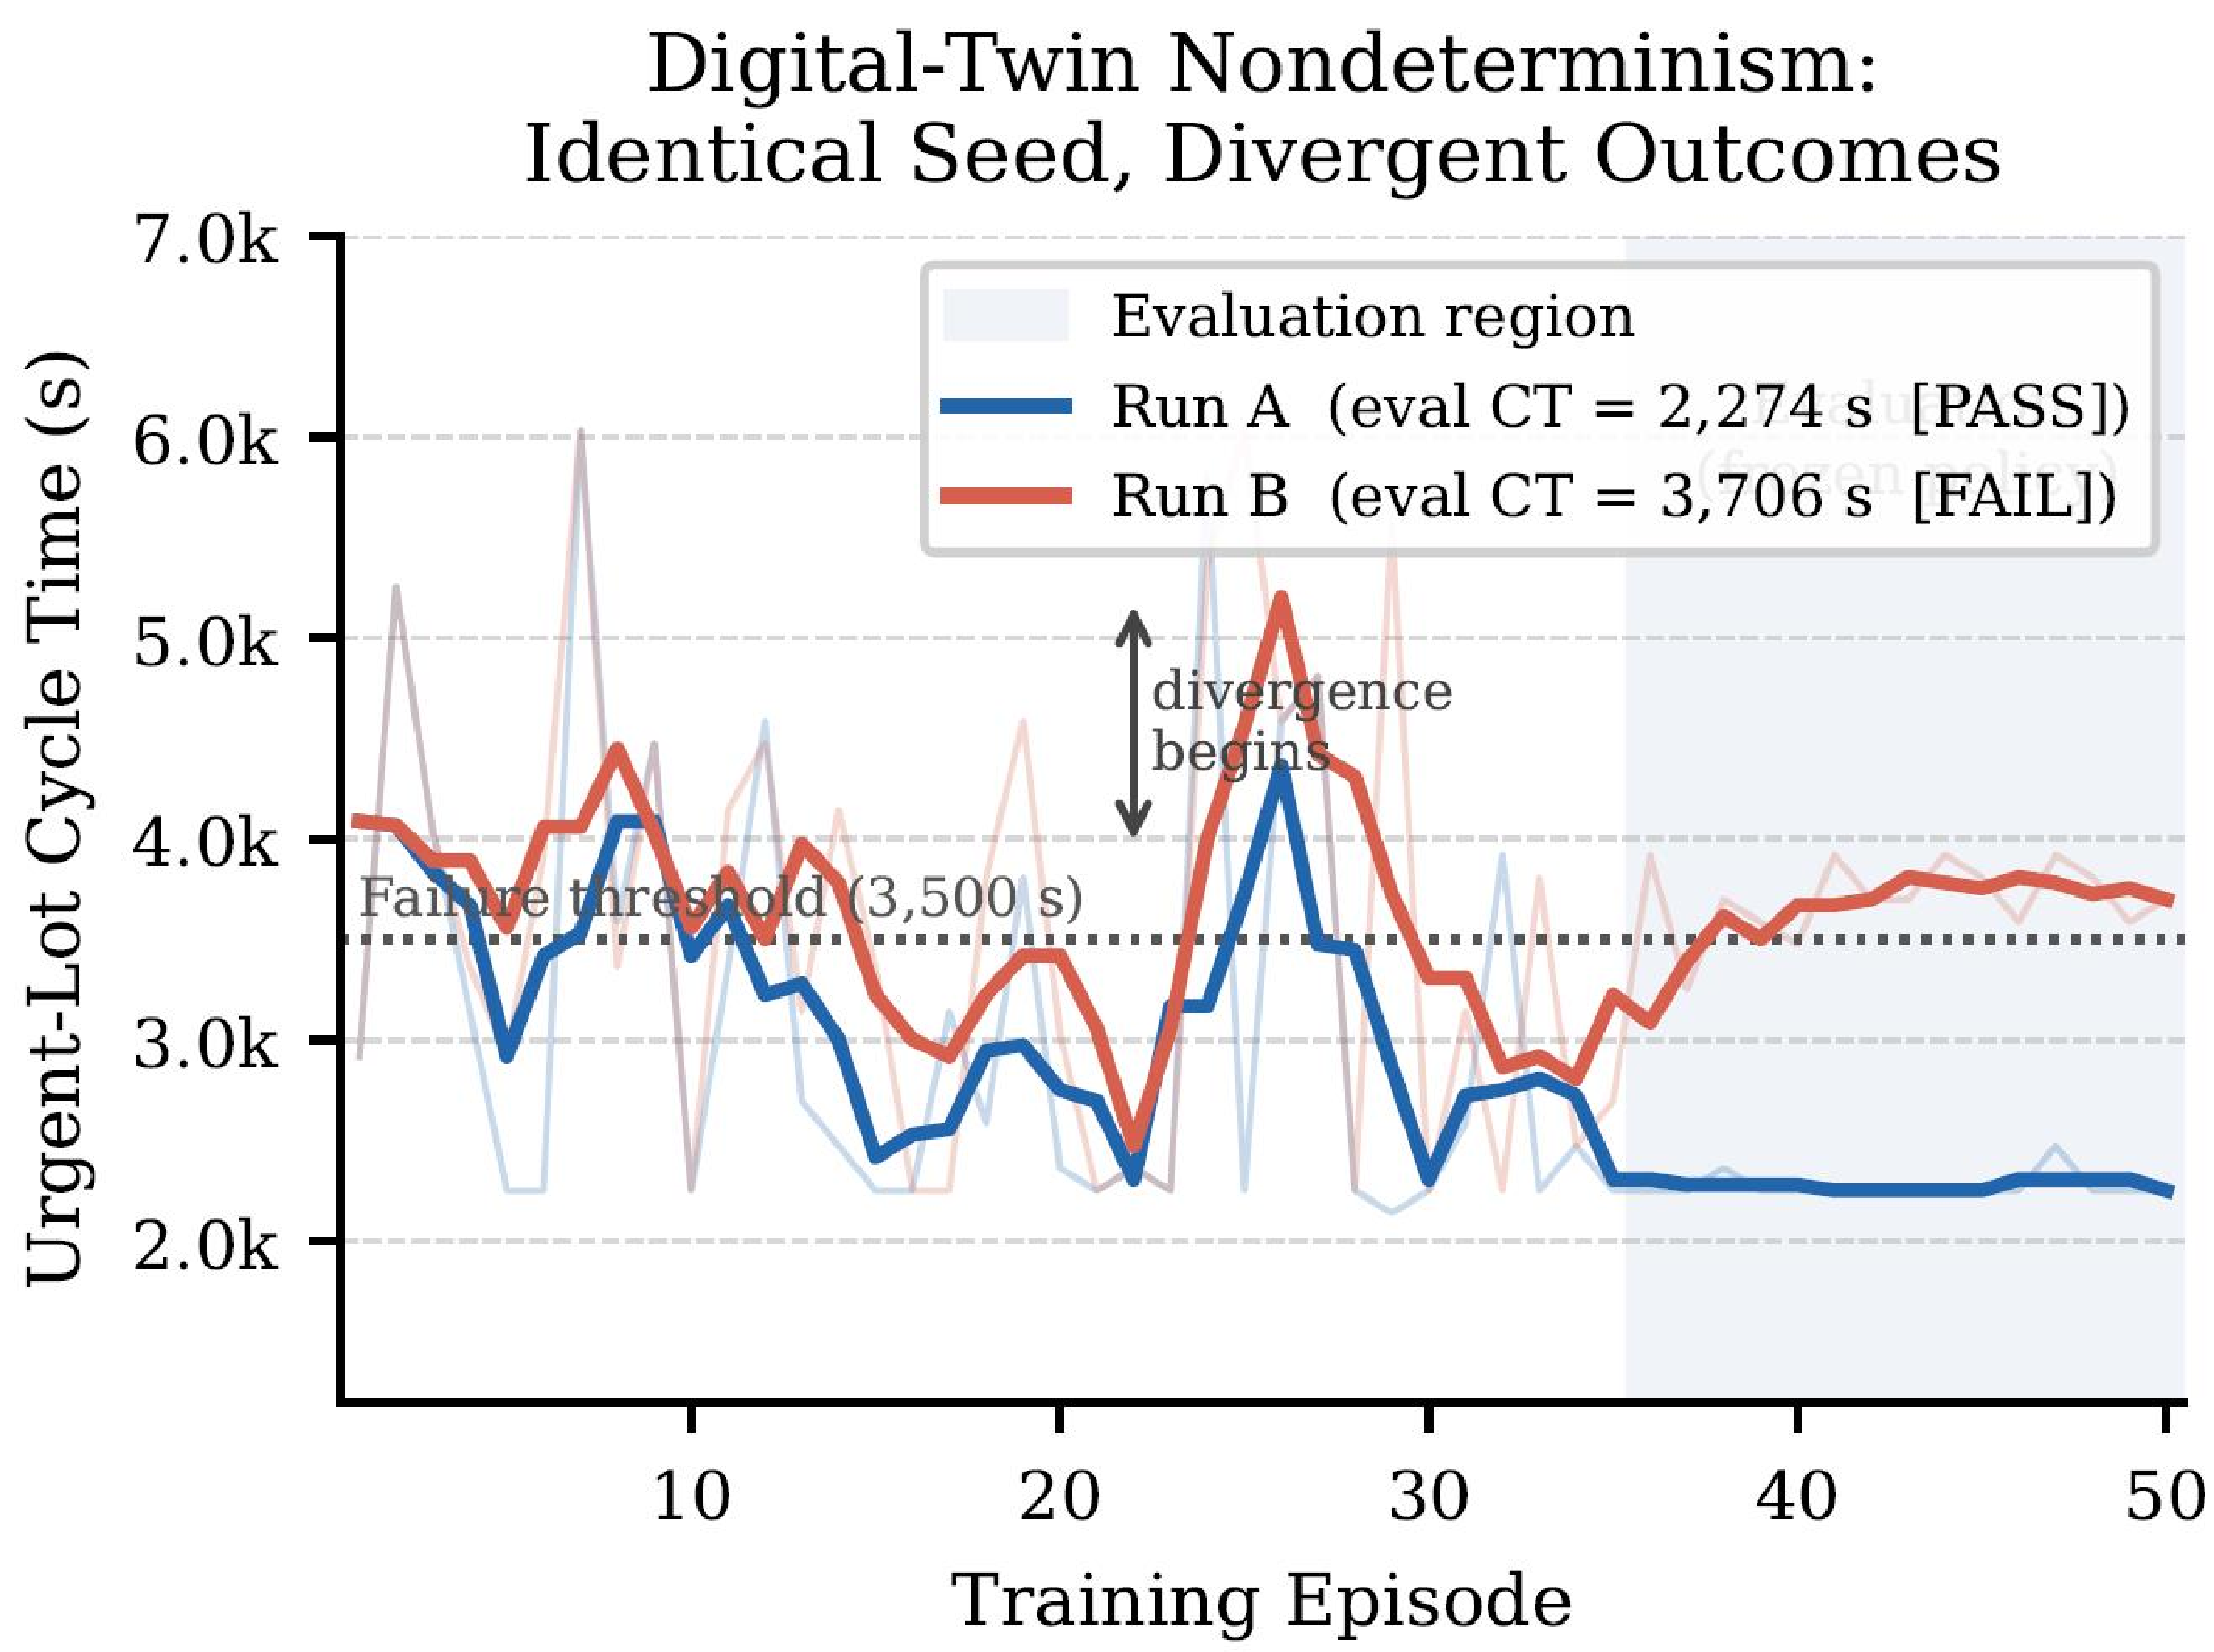
\includegraphics[width=0.98\columnwidth]{Figures/fig_nondeterminism.pdf}
  \caption{디지털 트윈 비결정성. \emph{동일한} 난수 시드와 설정을 가진 두 Pure DRL
  실행은 $\sim$20 에피소드 동안 거의 동일한 궤적을 공유하다가, Python RNG에 보이지
  않는 시뮬레이터 수준 타이밍 차이가 학습을 통해 증폭되면서 갈라진다: 하나는 통과
  정책으로, 다른 하나는 실패 정책으로 수렴한다. 따라서 고정 시드는 결과를 재현하지
  못하며, 이는 다수 시드에 걸친 분포적 보고를 정당화한다.}
  \label{fig:nondeterm}
\end{figure}

\paragraph{신뢰성 프로토콜.}
디지털 트윈이 내부적으로 비결정적이므로 고정 시드는 결과를 재현하지
못하며(그림~\ref{fig:nondeterm}), 다수의 독립 시드가 필요하다. 인과 사슬은 짧지만
중대하다: 시뮬레이터의 RNG 하위 타이밍 지터가 약간 다른 상태 전이를 낳고, 이것이
리플레이 버퍼에 들어가 적합된 $Q$-값을 교란하며, 학습에 걸쳐 누적되어 정책을 다른
끌개 분지(통과 또는 실패)로 밀어 넣을 수 있다(Laprie 분류의
\emph{결함}$\rightarrow$\emph{오류}$\rightarrow$\emph{실패} 사슬); 우리의 거버넌스
계층은 학습 중 이 사슬을 끊는다. RL의 분포적 보고 모범
사례 \citep{henderson2018,agarwal2021}에 따라, 각 조건을 $N{=}20$ 시드로 실행하고
단일 실행 평균이 아니라 실패율과 분산을 보고한다. 각 실행은 100 에피소드를
수행하며, 보상 곡선은 에피소드 70 이전에 안정화되므로(그림~\ref{fig:convergence})
마지막 30 에피소드(71--100)가 정착된 행동을 포착한다. 이 구간에서 룰은 동결되고
에이전트는 탐욕적으로 행동한다.

\paragraph{에이전트 설정.}
은닉층 [1024, 512, 256], 학습률 $3\times10^{-4}$, 할인율 $\gamma=0.98$, 리플레이
용량 100k, 멀티스텝 $n=3$, 타깃 갱신 300 스텝마다의 Rainbow DQN. 하이퍼파라미터는
표준 Rainbow 기본값 \citep{hessel2018}을 따르며 모든 조건에서 고정된다.

% ============================ 5. 주요 결과 ============================
\section{주요 결과}
\label{sec:results}

\begin{figure}[t]
    \centering
    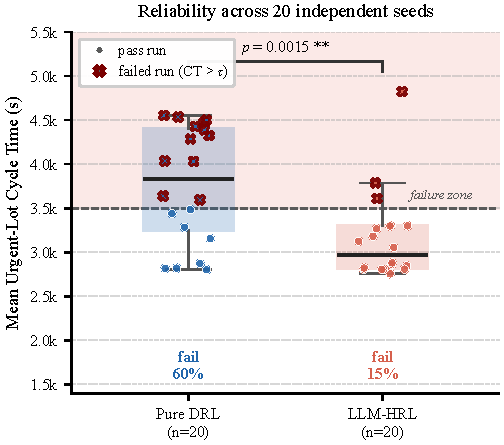
\includegraphics[width=0.86\columnwidth]{Figures/fig_reliability.pdf}
    \caption{20개 독립 시드에 걸친 신뢰성. 각 마커는 한 실행의 평균 평가 CT이며,
    $\times$는 치명적 실패 영역($\text{CT}>\tau$)의 실행을 표시한다. Pure DRL은
    실행의 60\%에서 실패하는 반면 LLM-HRL은 15\%에서 실패하며, 산포가 상당히
    작다($p=0.0015$, 이표본 $t$-검정).}
    \label{fig:reliability}
\end{figure}

\paragraph{LLM-HRL은 Pure DRL보다 신뢰성이 높다.}
그림~\ref{fig:reliability}은 핵심 결과를 보고한다. Pure DRL은 실행의 60\%(12/20)에서
치명적으로 실패하는 반면, LLM-HRL은 단 15\%(3/20)에서 실패하여 45\,\%p 감소한다.
평균 CT는 3{,}773\,s에서 3{,}148\,s로 감소하고($-625$\,s, $-16.6\%$), 산포가 뚜렷이
좁아진다(표준편차 656\,s\,$\to$\,492\,s). 차이는 유의하고 효과 크기도 크다: 시드별
평균에 대한 이표본 $t$-검정 결과 $t=-3.41$, $p=0.0015$, Cohen's $d=1.08$이며, CT
감소량의 95\% 신뢰구간은 $[253,997]$\,s, 실패율 감소량의 부트스트랩 95\% 신뢰구간은
$[20,70]$\,\%p다(실패율 자체의 Wilson 구간은 Pure DRL $[39,78]\%$, LLM-HRL
$[5,36]\%$). 생산 목표 달성률은 조건 간 통계적으로 동일하므로($p>0.05$), 거버넌스는
처리량을 희생하지 \emph{않고} 실패 꼬리를 제거한다.

\paragraph{개선의 본질은 실패 양상의 제거다.}
이득은 균일한 속도 향상이 아니라 Pure DRL의 실패 군집 제거로 이해하는 것이 가장
정확하다: 거버넌스 에이전트는 \emph{운 좋은} DRL 실행을 능가하지 않는다---둘 다
비슷한 사이클 타임에 도달한다---그러나 \emph{운 나쁜} 실행을 제거하여 거의 전체 결과
질량을 성공 군집으로 모은다. 그림~\ref{fig:convergence}은 학습 중 동일한 효과를
보인다: LLM-HRL 평균은 Pure DRL보다 아래에서 훨씬 좁은 $\pm$1\,SD 밴드로 추적하며,
실패 임계값 아래로 안정적으로 수렴한다.

\begin{figure}[t]
    \centering
    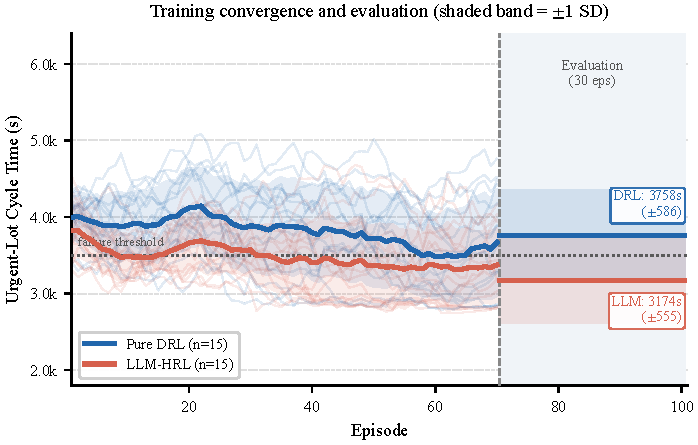
\includegraphics[width=0.98\columnwidth]{Figures/fig_convergence.pdf}
    \caption{100 에피소드에 걸친 학습 수렴(얇은 선: 개별 시드; 굵은 선: 평균; 음영
    밴드 $=\pm$1\,SD). 음영 영역(에피소드 71--100)은 동결 정책 평가 구간으로, 수평
    평균 선과 박스로 요약된다. Pure DRL은 높고 매우 가변적인 상태를 유지하며 실패
    임계값 위에 정착하고, LLM-HRL은 그보다 훨씬 아래의 낮고 안정적인 사이클 타임으로
    수렴한다. 둘 다 에피소드 70 이전에 안정화되어 평가 구간이 정착된 행동을 포착함을
    확인한다.}
    \label{fig:convergence}
\end{figure}

\paragraph{희소한 거버넌스가 학습된 정책을 형성한다.}
주목할 특성은, 평가 중 동결된 룰이 스텝의 2\% 미만에서 발동함에도 거버넌스
에이전트가 일관되게 신뢰 가능하다는 점이다. 이는 거버넌스의 가치가 \emph{얼마나
자주}가 아니라 \emph{언제} 개입하는가에 있음을 시사한다: 학습 중 잘 맞춰진 소수의
마스킹---긴급 로트가 있고 긴급 로트 행동을 취해야 할 때---이 Pure DRL이 운으로만
획득하는 행동을 에이전트에게 가르친다. 거버넌스는 런타임 필터링이 아니라 학습 궤적을
교정한다.

\subsection{충돌 영역에 걸친 일반화}
\label{sec:sweep}
이 이득이 단일 운영점에 특화된 것일까? 이를 확인하기 위해 긴급 로트 밀도를
세 영역---전체 로트의 1.6\%, 4.7\%, 7.7\%---으로 변화시키며 두 조건을
측정한다(그림~\ref{fig:sweep}). 낮은 밀도(1.6\%)에서는 긴급 로트가 병목을 두고
경합하는 일이 드물어 두 기법 모두 거의 동일한 사이클 타임으로 성공한다: 거버넌스는
필요하지도, 해롭지도 않다. 밀도가 높아지면 충돌이 심화되어 Pure DRL이 실패하기
시작하며---4.7\%와 7.7\% 모두에서 60\% 실패율에 도달---LLM-HRL은 모든 영역에서
실패율을 엄격히 더 낮게(0\%, 40\%, 15\%) 유지하고 사이클 타임을 $\tau$ 아래 또는
근처로 유지한다. 따라서 거버넌스 마진은 \emph{충돌 밀도와 함께 증가}하며, 이는 자원
부담이 가장 큰 지점과 정확히 일치한다. 이는 신뢰 가능한 거버넌스가 임팩트를 발휘하는
영역을 식별하고, 그 효과가 단일 설정의 산물이 아님을 보인다.

\begin{figure}[t]
    \centering
    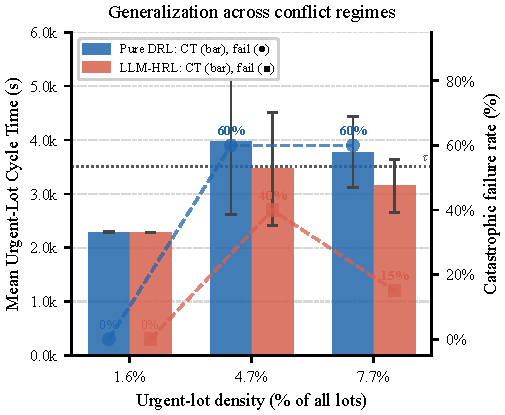
\includegraphics[width=0.92\columnwidth]{Figures/fig_sweep.pdf}
    \caption{긴급 로트 충돌 영역에 걸친 일반화(막대: 평균 CT, $\pm$1\,SD; 점선:
    치명적 실패율). 낮은 밀도에서는 두 기법 모두 성공하지만, 충돌이 심화되면 Pure
    DRL은 실패하는 반면 LLM-HRL은 모든 영역에서 실패율을 엄격히 더 낮게 유지한다.
    거버넌스 이득은 충돌 밀도와 함께 증가한다.}
    \label{fig:sweep}
\end{figure}

% ============================ 6. 절제 연구 ============================
\section{절제 연구: 무엇이 거버넌스를 작동하게 하는가?}
\label{sec:ablation}

주요 결과는 LLM 거버넌스가 도움이 된다는 \emph{사실}을 확립한다. 본 절은 \emph{이유}를
분리한다. 우리의 전체 기법은 세 가지 속성을 결합한다: \emph{하드}(보상이 아닌 마스크),
\emph{맥락적}(KPI 조건부), \emph{적응적}(매 에피소드 수정)인 행동 제약. 우리는 한
번에 정확히 하나의 속성을 제거하여 각각을 시험하며, 보상 함수와 L0 에이전트를 고정한
채 20 시드 전체 모델 및 Pure DRL 앵커와 대조하여 변형당 5개 시드를 보고한다.
그림~\ref{fig:ablation}은 모든 조건을 요약한다.

\begin{figure*}[t]
    \centering
    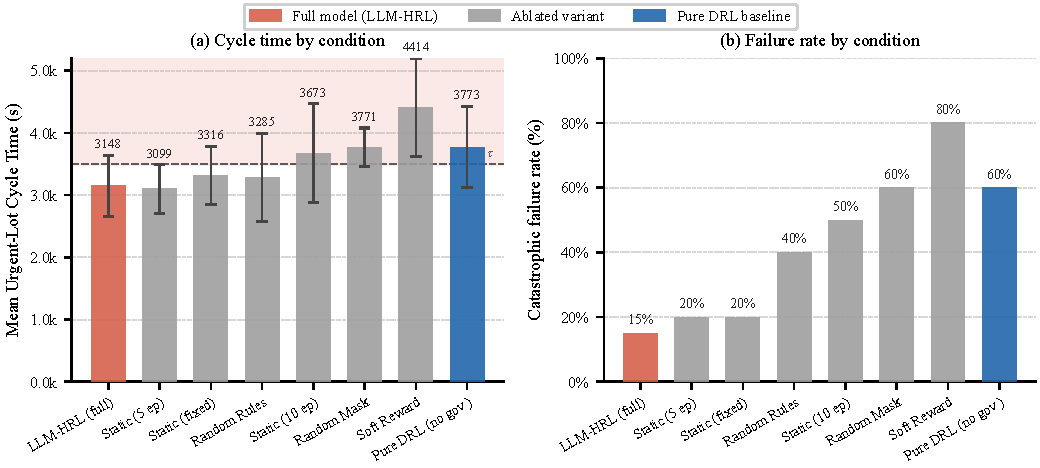
\includegraphics[width=0.92\textwidth]{Figures/fig_ablation.pdf}
    \caption{단일 축 절제(시드별 결과의 평균; 오차 막대 $=\pm$1\,SD; 절제 변형은 5
    시드 파일럿, 전체 모델과 Pure DRL은 20 시드). 각 절제 변형은 전체 모델의 속성 하나를
    정확히 제거한다. \textbf{(a)} 평균 사이클 타임; 음영 영역은 실패
    영역($\text{CT}>\tau$). \textbf{(b)} 치명적 실패율. 하드 마스크 제거(Soft
    Reward)는 거버넌스 없는 DRL보다 나쁘고, 맥락 제거(Random Mask)는 거버넌스 없는
    DRL보다 낫지 않으며, 적응성 제거(Rule-Based)는 전체 모델의 평균 사이클 타임에
    필적하지만 실행의 60\%에서 실패한다. 전체 모델만이---하드하고 맥락적이며
    적응적---낮은 사이클 타임과 낮은 실패율을 동시에 달성한다.}
    \label{fig:ablation}
\end{figure*}

\paragraph{하드함 제거: 마스크 $\to$ 보상 정형화.}
L1 행동 마스크를, 마스크가 금지할 행동과 동일한 행동에 페널티를 주는 동등한
\emph{보상 정형화} 항으로 대체하여 거버넌스 신호는 동일하되 ``소프트''하게 만든다. 이
\emph{Soft Reward} 변형은 우리가 시험한 최악의 조건이다: 평균 CT가 4{,}414\,s,
실패율 80\%로---\emph{거버넌스 없는 Pure DRL(3{,}773\,s, 60\%)보다 나쁘고}, 제안
기법보다 유의하게 나쁘다($p<0.001$). 이유는 시사적이다: 충돌 시점에 지배하기에
충분히 큰 정형화 항은 훨씬 더 빈번한 비충돌 구간도 왜곡하여, 학습을 불안정하게 하는
비정상적 목표를 주입한다. 하드 마스킹은 룰이 발동할 때만 행동을 가지치기하고 보상은
왜곡하지 않음으로써 이를 회피한다. \emph{거버넌스의 이득은 하드 제약이지, 그것이
인코딩하는 신호가 아니다.}

\paragraph{맥락 제거: 조건부 $\to$ 무작위 마스킹.}
다음으로 \emph{어떤} 행동 제약이든 충분한지 묻는다. \emph{Random Mask} 변형은
LLM-HRL과 동일한 평균 빈도의 마스크를 적용하되, KPI를 완전히 무시하고 무작위
에피소드의 무작위 행동에 적용한다. 이는 실행의 60\%에서 실패하며(제안 기법 15\% 대비,
$p<0.05$), 평균 CT 3{,}771\,s로 거버넌스 없는 DRL과 사실상 구별되지 않는다. 행동
공간을 제약하는 것은 제약이 \emph{올바른 맥락}에서 적용될 때만 도움이 된다: 잘못된
행동을, 혹은 잘못된 시점에 마스킹하는 것은 신뢰성 이득을 주지 못한다. \emph{제약이
언제 발동하는가는 제약이 존재한다는 사실만큼 중요하다.}

\paragraph{적응성 제거: 에피소드 단위 $\to$ 고정 룰.}
마지막으로 에피소드 수정의 가치를 \emph{Rule-Based} 변형으로 시험한다: LLM-HRL과
동일한 L1 집행과 L0 에이전트를 쓰되, LLM 수정 없이 고정된 수작업 룰(긴급 로트가 둘을
초과하여 대기할 때 비긴급 행동을 금지)로 구동된다. 이는 가장 시사적인 비교다.
\emph{평균적으로는} 제안 기법에 거의 필적한다(평균 CT 3{,}347\,s 대 3{,}148\,s; 차이는
유의하지 않음, $p=0.43$)---이는 고정 룰이 ``충분히 좋다''고 시사할 수 있다. 그러나
여전히 실행의 60\%에서 실패하며, 개별 평가 에피소드는 8{,}567\,s까지 치솟는다. 정적
룰은 긴급 충돌이 발생하지 않는 에피소드에서도 탐색을 제약하여, 보상 정형화와 마찬가지로
정책을 지속적으로 왜곡한다. 이는 Pure DRL이 여전히 가끔 찾아낼 수 있는 운 좋은 궤적을
차단하여, 구조적으로 더 나쁜 실패를 남긴다. \emph{평균을 맞추는 것은 꼬리를 제거하는
것과 다르다---꼬리를 제거하는 것은 적응이다.}

\paragraph{요약.}
단일 축 절제는 명확한 판정을 준다: 세 속성---하드함, 맥락성, 적응성---각각이
필수적이며, 어느 하나라도 제거하면 신뢰성이 거버넌스 없는 60--80\% 실패 영역으로
붕괴한다. 전체 모델은 낮은 사이클 타임과 낮은 실패율을 동시에 달성하는 유일한
조건이다(그림~\ref{fig:ablation}). 특히 LLM의 가치는 이 세 속성을 한꺼번에, 수작업
없이 자동으로 공급하면서 모든 룰에 사람이 읽을 수 있는 근거를 부여한다는 점에 있다.

% ============================ 7. 논의 ============================
\section{논의}
\label{sec:discussion}

우리 결과는 LLM-over-DRL 거버넌스가 \emph{무엇을 위한} 것인지 재정의한다. 거버넌스
에이전트는 운 좋은 Pure DRL 실행을 이기지 않는다. 그 가치는 운 나쁜
실행---디지털 트윈 비결정성에서 간헐적으로 발생하는 치명적 스케줄---을 제거하는 데
있다. 하나의 잘못 스케줄된 긴급 로트가 품질시간 위반과 수율 손실로 연쇄될 수 있는
제조에서, 실패 꼬리를 제거하는 것은 한계 평균 개선보다 가치가 크다. 이는 기여를
신뢰성 공학 \citep{avizienis2004}과 정렬시킨다: \emph{결함}은 관측 불가능한
시뮬레이터 비결정성이고, \emph{오류}는 결함이 학습을 손상시킬 때 긴급 로트를 덜
우선시하는 정책이며, \emph{실패}는 $\overline{\mathrm{CT}}>\tau$다. 거버넌스는
\emph{내결함성 메커니즘}이다: 고전적 내결함 시스템에서 중복성이 하듯, 학습 중 정책을
유도하여 결함$\to$오류$\to$실패 사슬을 끊는다.

절제 연구는 이를 실행 가능한 설계 원칙으로 다듬는다: 이득은 LLM 자체도, 어떤 외부
신호의 주입도 \emph{아니라} 안전하지 않은 행동의 \emph{하드하고 맥락적이며 적응적인}
가지치기다. 이를 제공하는 오버헤드는 미미하다: 에피소드당 1회 LLM
호출($\approx$2--5\,s), 2--4개 룰, 스텝당 마이크로초 단위 L1 평가.

\paragraph{왜 LLM이고, 수작업 룰이 아닌가?}
핵심 요소가 하드하고 맥락적이며 적응적인 마스킹인데, 왜 룰을 직접 작성하지 않는가?
Rule-Based 결과가 답한다: 고정 전문가 룰은 충돌 패턴이 변할 때 \emph{적응}하지 못해
60\%의 경우에 실패하며, 수작업으로 적응성을 복원하려면 충돌 영역과 제품 믹스마다 룰
집합을 재설계해야 한다---룰 기반 디스패치가 악명 높은 취약한 수작업이다. 비-LLM \emph{적응형}
생성기(온라인 의사결정트리, 임계값 최적화기, 베이지안 룰 갱신기)도 원칙적으로 같은
적응성을 줄 수 있으나, 대개 수작업 특징 공간을 요구하고 라인마다 재튜닝해야 하며
불투명한 파라미터를 내놓는다; LLM은 대신 적응적·맥락적·\emph{감사 가능}한 룰을 자연어
지식으로부터 제로샷으로, 생산 데이터를 외부에 노출하지 않고 로컬로 공급한다. 직접
비교는 향후 과제로 남긴다.

\paragraph{제조를 넘어서.}
프레임워크의 어떤 부분도 반도체에 특화되어 있지 않다. 이를 가치 있게 만드는
조건---실행 간 정책 비신뢰성을 유발하는 확률적 환경, 그리고 잘못 처리하면 평균
처리량보다 훨씬 큰 손실을 내는 드물지만 비용이 큰 사건---은 신호등 제어, 창고 및 잡샵
스케줄링, 클라우드 자원 할당, 응급 디스패치에서도 반복된다. 각 경우에서, 태스크 수준
KPI를 읽고 하드하고 맥락적이며 감사 가능한 제약을 내보내는 LLM은 재학습 없이 기존 DRL
제어기를 견고하게 만들 수 있다. 따라서 우리는 본 기여를 신뢰 가능한 RL을 위한 일반적
레시피로 보며, 반도체 스케줄링은 그 경계가 아니라 까다로운 한 사례다.

\paragraph{배포 및 자원 함의.}
본 접근법은 배포에 실용적이다: 재학습 없이 기존 에이전트에 신뢰성을 더하고, 생산
데이터가 공장을 떠나지 않도록 보급형 하드웨어에서 로컬로 동작하며, 모든 결정을
운영자가 검토·재정의할 수 있는 언어로 노출한다. 자원 임계적 공장에서는 추가 이점이
있다---치명적 꼬리가 Q-time 위반·스크랩·재작업이 집중되는 지점이므로, 그것을 제거하면
위험 로트에 체화된 에너지·물·소재도 보전된다. 따라서 향상된 신뢰성은 운영적 이점과
더불어 직접적인 자원 효율 이득을 수반한다.

% ============================ 8. 한계 ============================
\section{한계}
\label{sec:limitations}

모든 실험은 시뮬레이션 내에서 수행되었다. 실제 배포는 실시간 설비 인터페이스와
형식적 안전 검증을 필요로 하며, 제품·공장에 걸친 일반화는 디지털 트윈 재보정을
요구한다. 절제 변형은 각각 5개 시드를 사용하므로 시드별 평균 차이를 $t$-검정에만
의존하기보다 실패율 및 최악 에피소드와 함께 제시한다. 무엇보다, 우리는 LLM을
\emph{적응형 비-LLM} 룰 생성기(예: 온라인 의사결정트리, 임계값 최적화기)와 비교하지
않는다; 그것들이 LLM의 제로샷·감사 가능한 룰에 필적할 수 있는지가 핵심 다음 실험이다.
끝으로, 한 시드에서 학습/평가 분포 이동으로 최종 룰이 발동하지 않아 그 실행이 사실상
Pure DRL이 되었다; 더 강한 모델이나 분포에 강건한 임계값이 도움이 될 수 있다.

% ============================ 9. 결론 ============================
\section{결론}

우리는 LLM을 정책 생성기가 아니라 비결정성으로 유발되는 치명적 실패에 맞서 기성 DRL
에이전트를 견고하게 만드는 적응형 거버넌스 모듈로 취급했다. 실제 공장 데이터로 구축된
반도체 디지털 트윈에서의 긴급 로트 스케줄링에서, 처리량을 해치지 않으면서 치명적
실패율을 60\%에서 15\%로, 평균 사이클 타임을 625\,s 감소시키며($p<0.01$, $N{=}20$
시드) 충돌 영역에 걸쳐 일관된다. 단일 축 절제 연구는 이득을 \emph{하드하고 맥락적이며
적응적인} 행동 제약으로 국소화한다: 보상 정형화는 거버넌스 없는 경우보다 나쁘고($p<0.001$),
무조건적 마스킹은 낫지 않으며, 고정 룰은 평균은 맞추지만 실패 꼬리를 그대로 남긴다.
공장에서 이것이 가져오는 자원 절감---더 적은 스크랩 소재---을 넘어, 더 넓은 기여는
LLM-over-DRL 거버넌스를 \emph{신뢰 가능한} 강화학습을 위한 일반적·로컬·감사 가능한
메커니즘으로 재정의하는 데 있다.

\bibliography{references}

\end{document}
